\section{Security Evaluation}\label{sec:eval}

\subsection{Methodology}
The evaluation is automated. A \texttt{Lab} builds a fresh in-process server
(with a controllable clock) for each run; a \texttt{VirtualPhone} plays the
authenticator using \texttt{tba\_core}; and a \texttt{Mitb} object rewrites
requests and QR codes exactly as the live \texttt{mitmproxy} addon does. Two user
models bound the human: an \emph{attentive} user approves only when the phone's
display matches their intent (and always approves when the phone shows nothing,
as in blind signing), while a \emph{careless} user always approves. Thirteen
scenarios (S1--S13) are run in all four modes and each outcome is compared with a
pre-declared expected value; \texttt{make scenarios} exits non-zero on any
mismatch. All results below are the committed output of \texttt{make eval} and
live in \texttt{results/}.

Not every scenario is an end-to-end HTTP test. S5 and S12 exercise the Python
cryptographic and encoding library (\texttt{tba\_core}) directly --- tampering
with each transaction field after a code is issued, and feeding malformed QR
payloads. S8 tests the confirmation logic with separate SQLite connections across
concurrent threads. S13 drives the HTTP confirmation endpoint with malformed
signatures. The remaining scenarios run against the in-process server.

\subsection{Case study: man-in-the-browser}
\Cref{fig:mitb} shows the live attack through \texttt{mitmproxy}, for a transfer
the user meant to send to \textbf{TRAN THI B (0123456789)}. The malware rewrites
the recipient to \textbf{LE VAN M (0999888777)}, the attacker's account, and
masks the bank's confirmation page so the laptop still shows TRAN THI B. The
phone, which reads the transaction the server actually holds, tells the truth: in
\texttt{hmac} and \texttt{sig} it shows LE VAN M, so an attentive user rejects; in
\texttt{sig\_blind} it shows no details, so the user approves the theft.

\begin{figure}[htbp]
\centering
\begin{minipage}{0.3\linewidth}\centering
  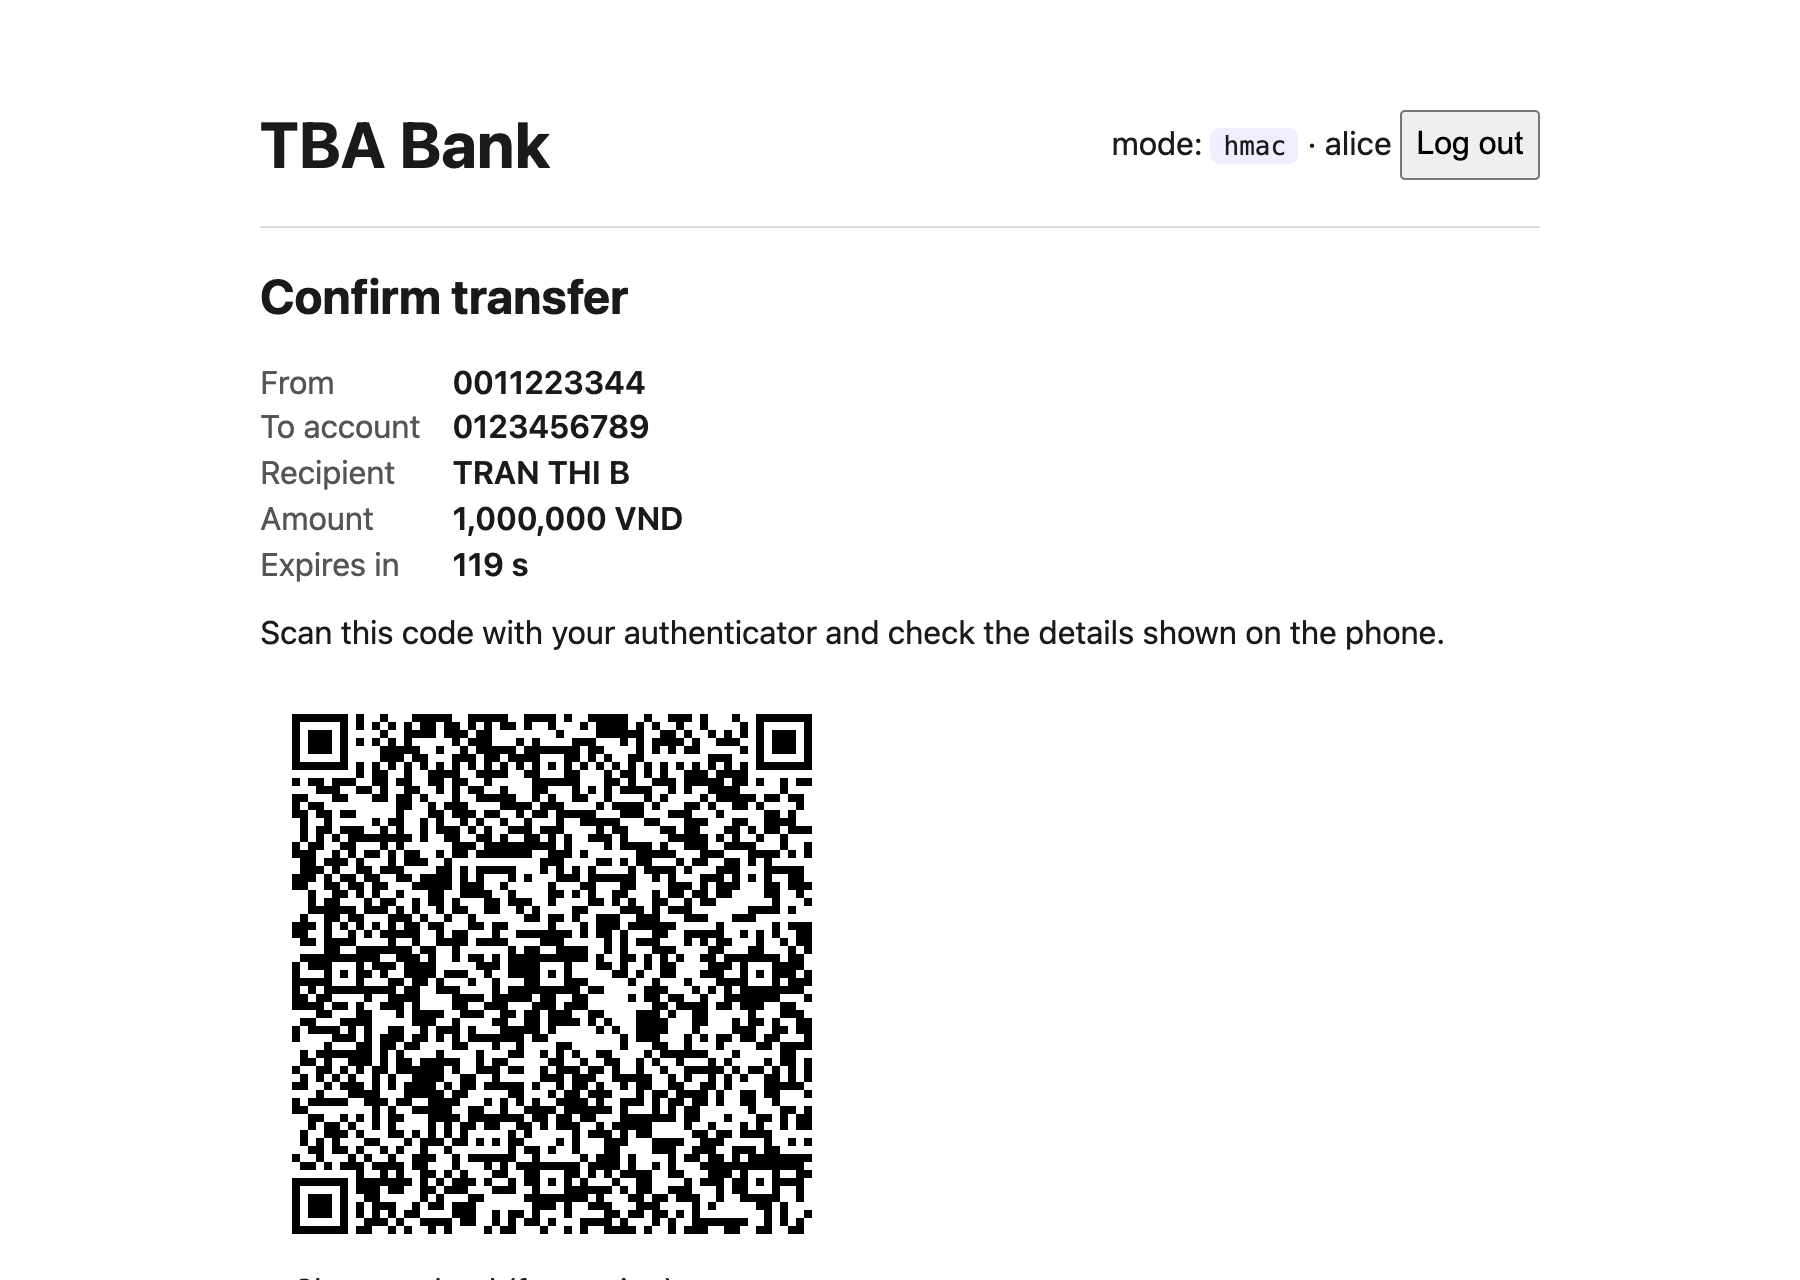
\includegraphics[width=\linewidth]{figures/hmac_laptop.png}\\[1mm]
  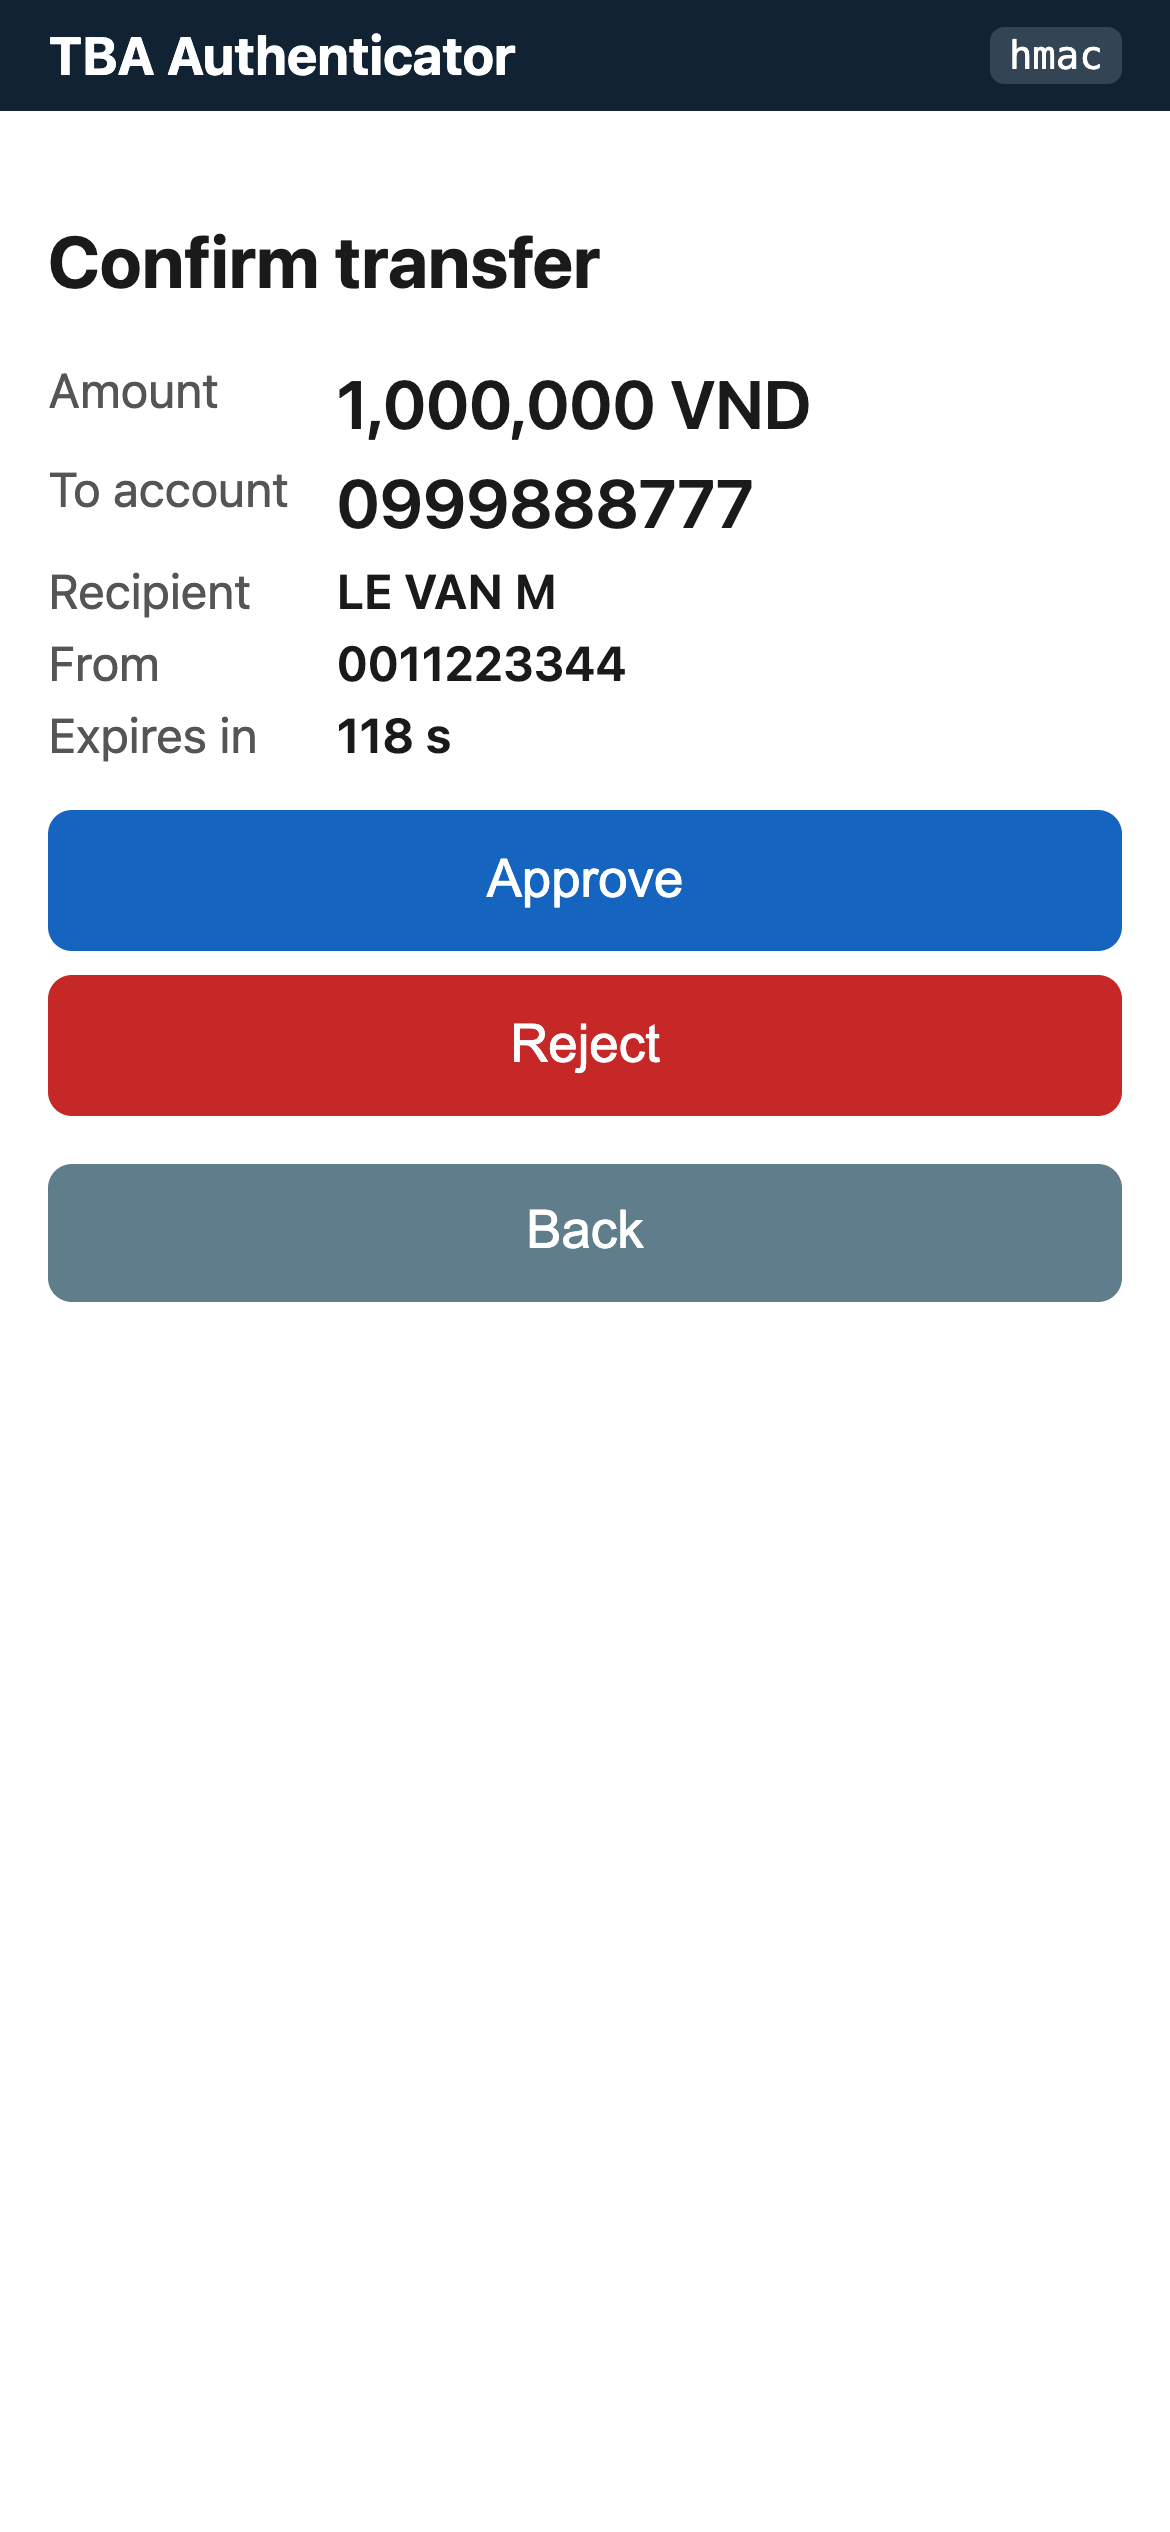
\includegraphics[height=3.4cm]{figures/hmac_phone.png}\\ \footnotesize\texttt{hmac}
\end{minipage}\hfill
\begin{minipage}{0.3\linewidth}\centering
  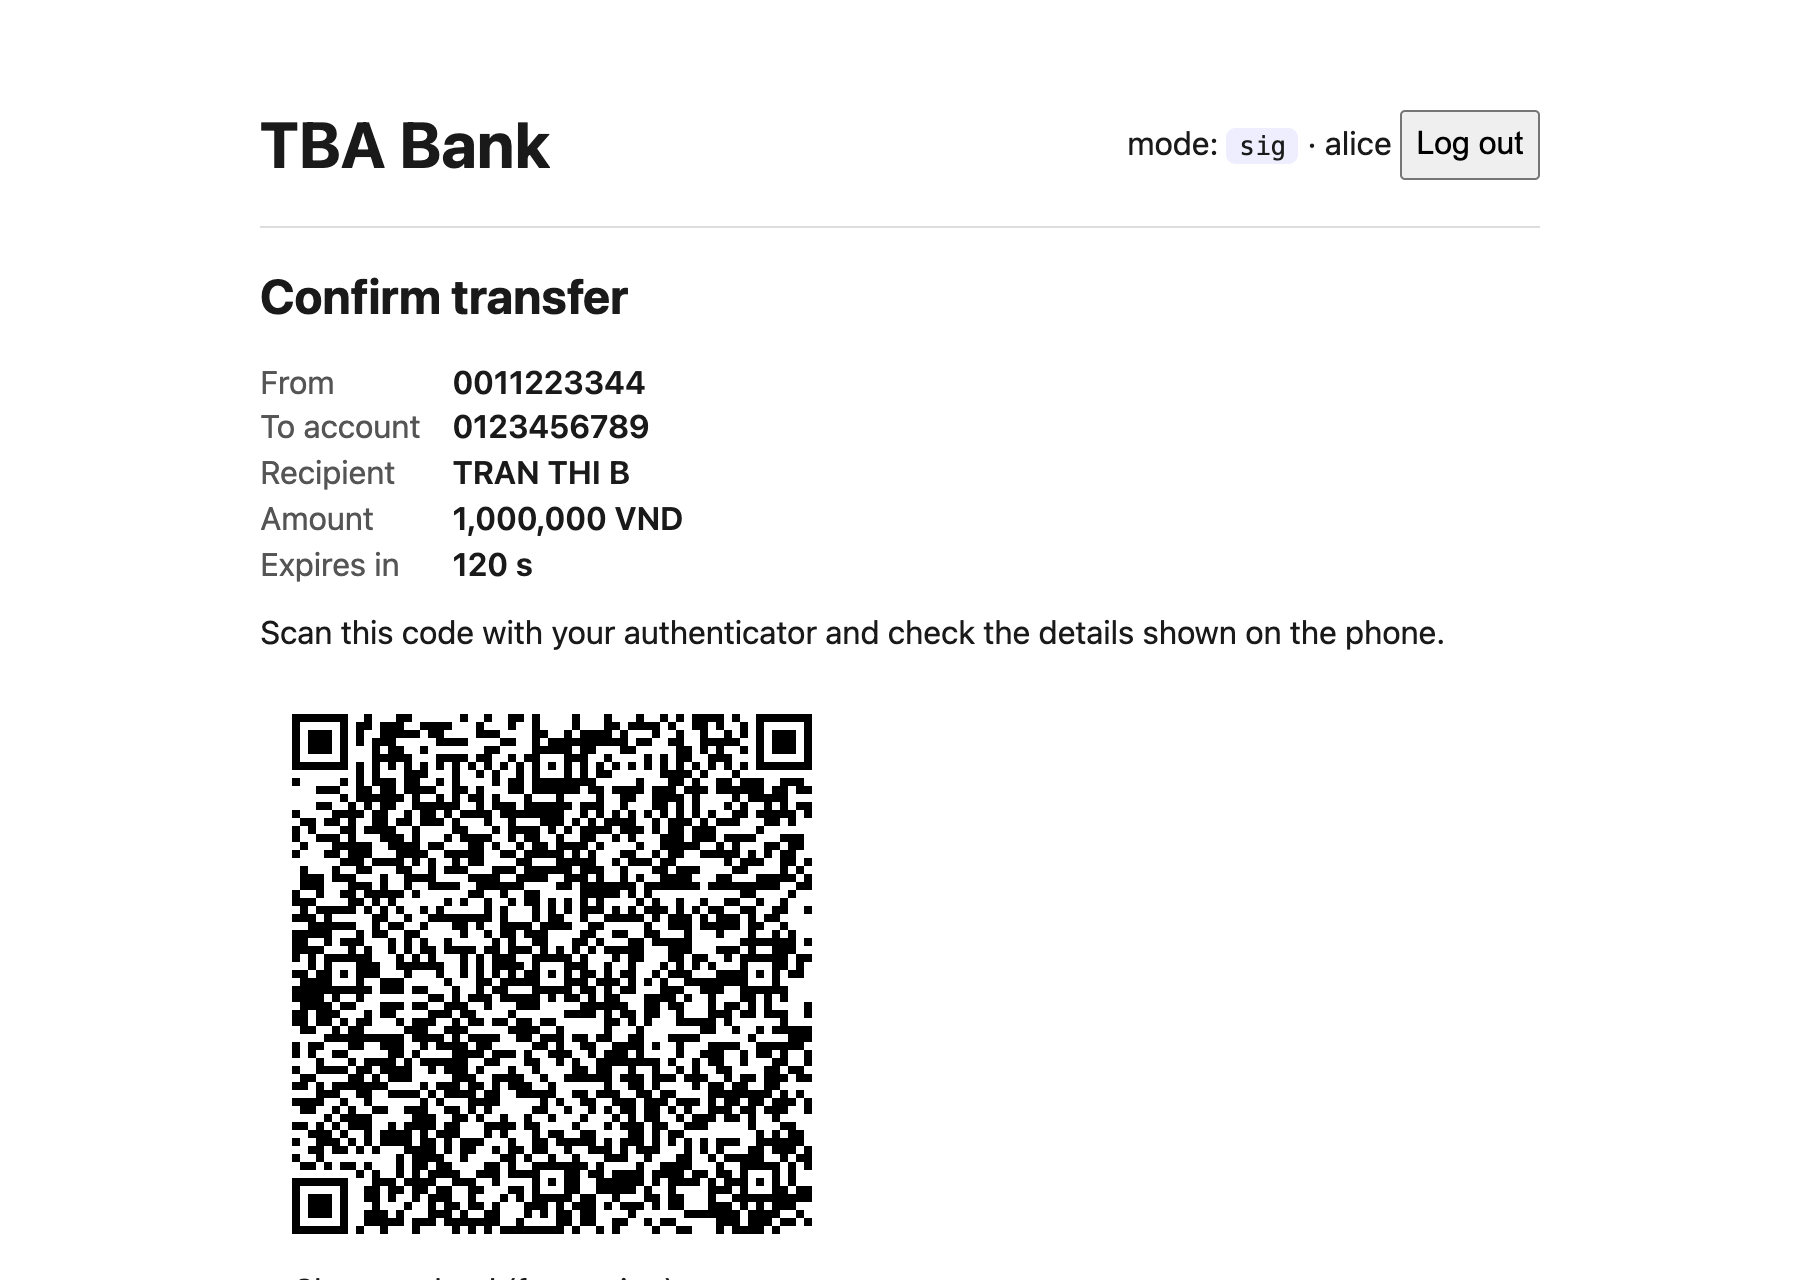
\includegraphics[width=\linewidth]{figures/sig_laptop.png}\\[1mm]
  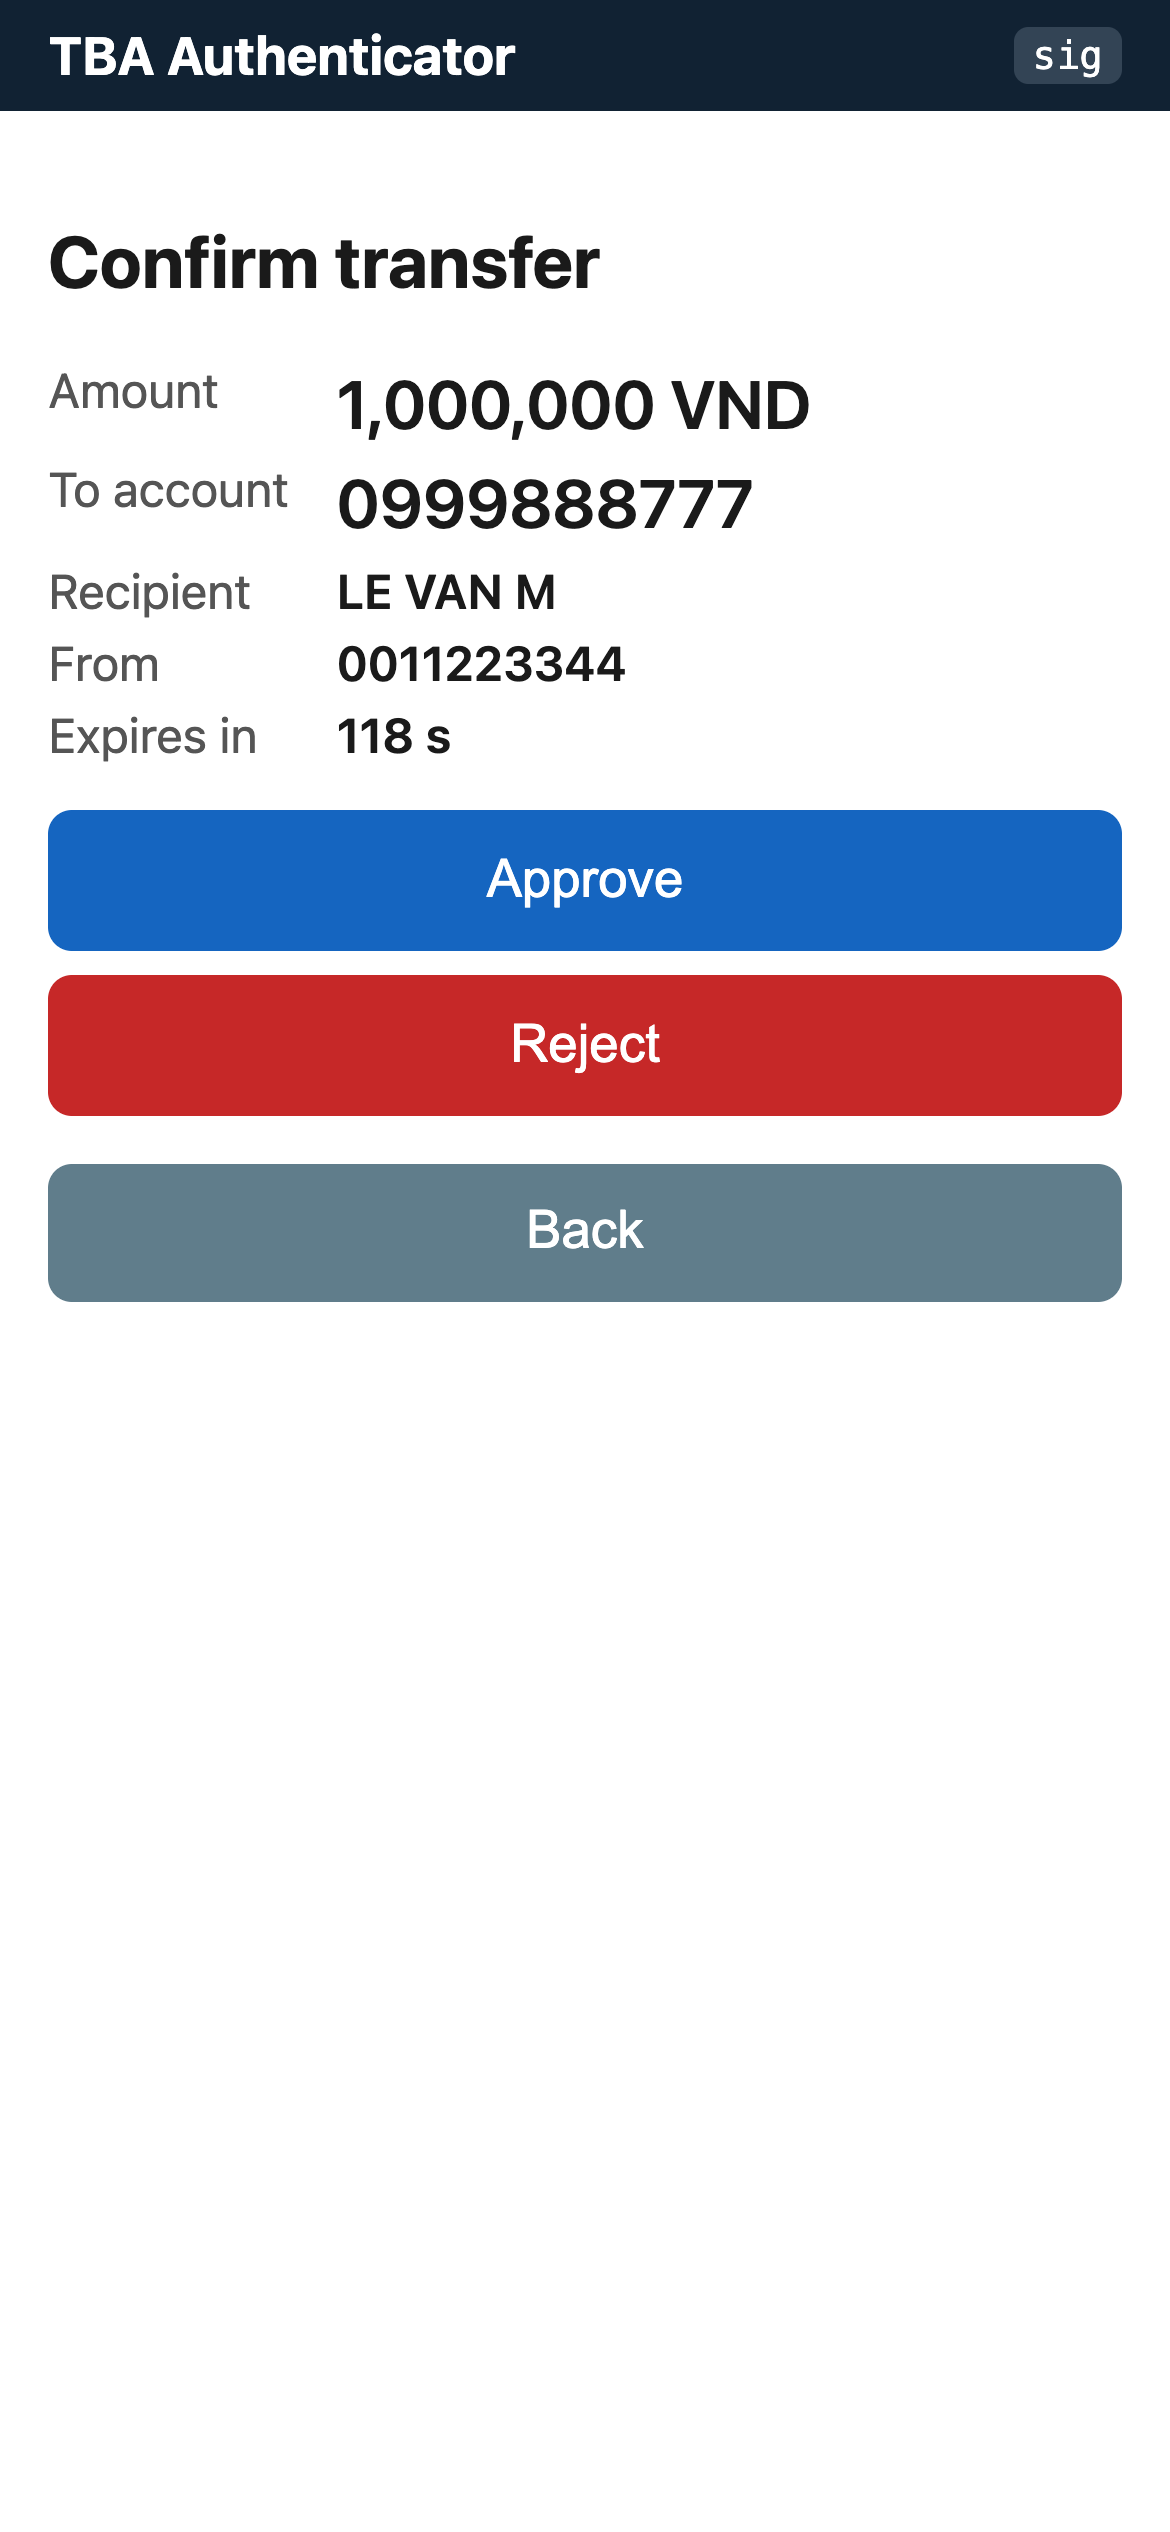
\includegraphics[height=3.4cm]{figures/sig_phone.png}\\ \footnotesize\texttt{sig}
\end{minipage}\hfill
\begin{minipage}{0.3\linewidth}\centering
  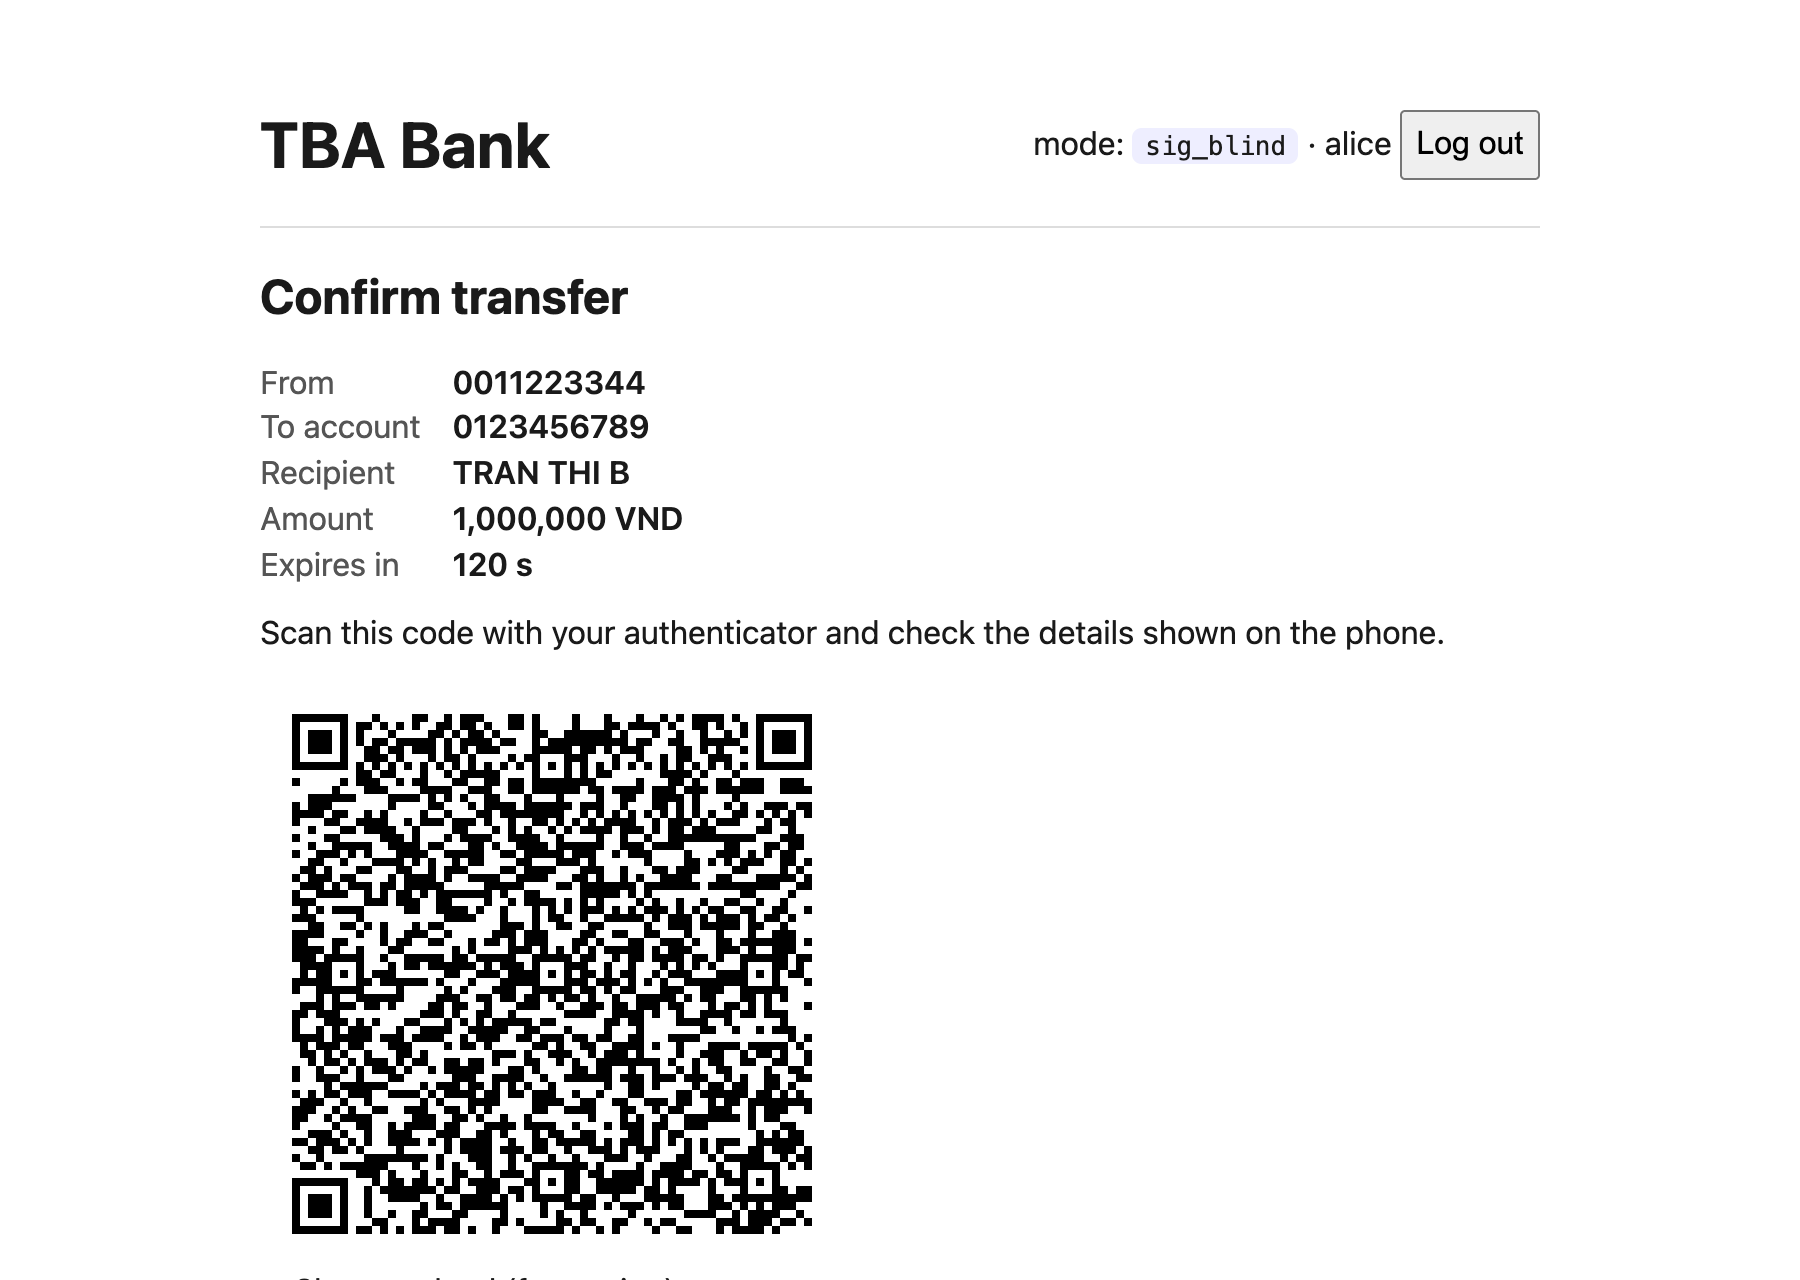
\includegraphics[width=\linewidth]{figures/sig_blind_laptop.png}\\[1mm]
  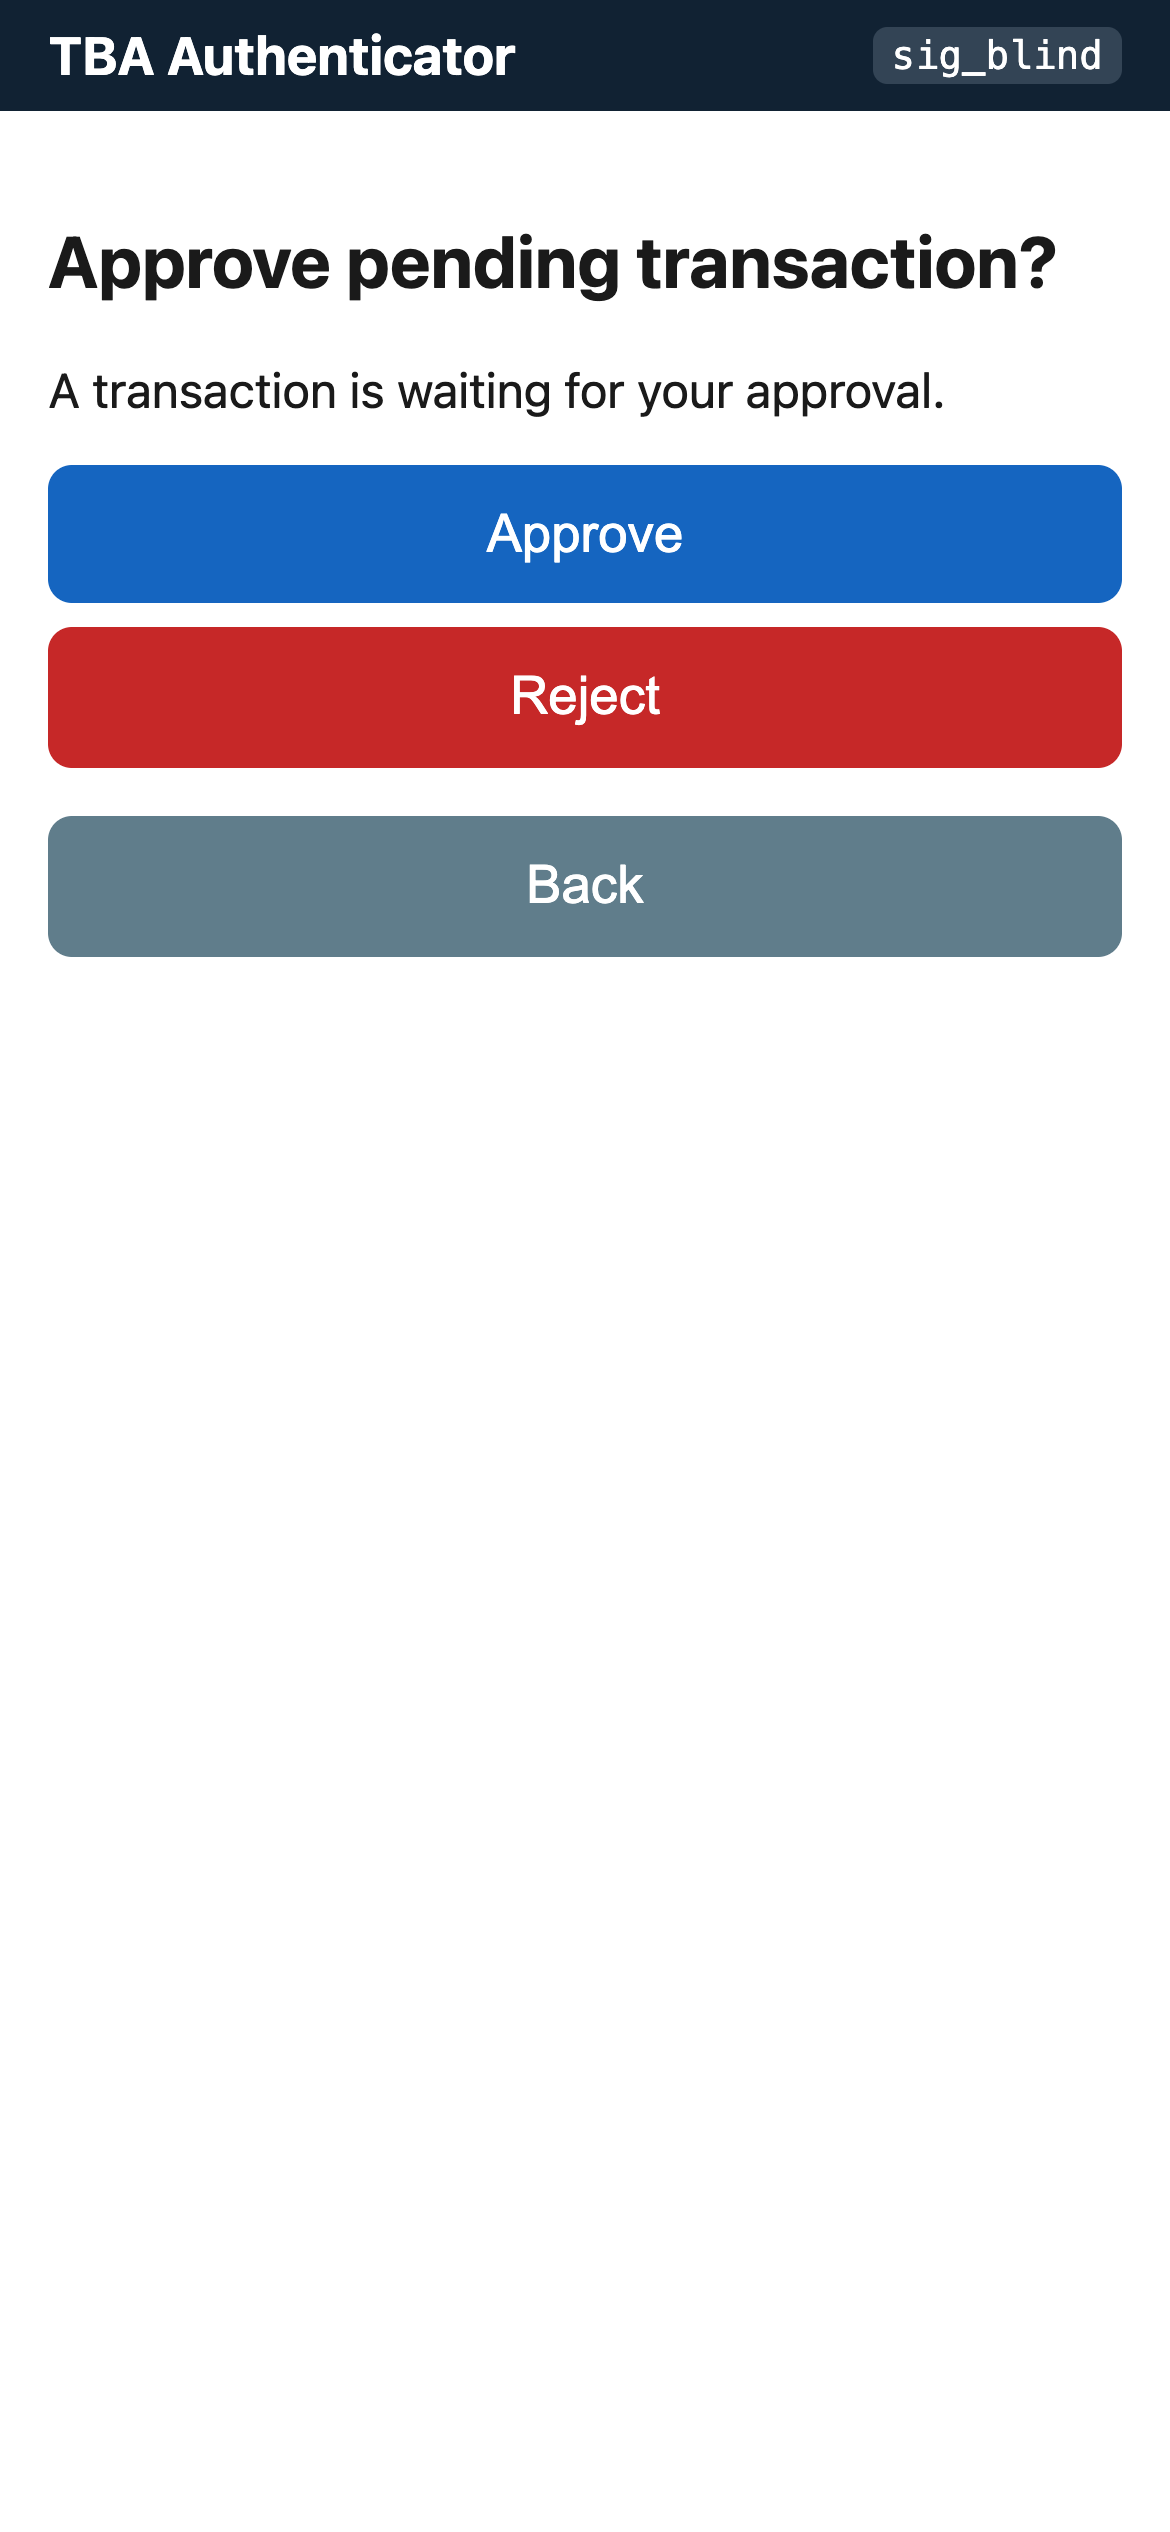
\includegraphics[height=3.4cm]{figures/sig_blind_phone.png}\\ \footnotesize\texttt{sig\_blind}
\end{minipage}
\caption{Live man-in-the-browser (F4). Top row: the laptop confirmation page,
deceived into showing TRAN THI B in every mode. Bottom row: the phone. In
\texttt{hmac}/\texttt{sig} the phone shows the real recipient (0999888777, LE VAN
M); in \texttt{sig\_blind} it shows no details at all.}
\label{fig:mitb}
\end{figure}

\subsection{Scenario results}
\Cref{tab:scenarios} in the main text is the full matrix (generated by \texttt{make scenarios};
\cmark{} = secure outcome, \xmark{} = insecure outcome, \texttt{--} = not
applicable). The measured outcomes equal the expected outcomes in all $56$ cells.

The matrix answers the research questions directly. Binding the code to the
transaction (\texttt{hmac}, \texttt{sig}) blocks the recipient and amount swaps
(S2a, S3) that \texttt{baseline} lets through, and both block tampering with any
field after the code is issued (S4, S5) --- this is RQ1. The difference between
\texttt{hmac} and \texttt{sig} appears in S10 and S11 (RQ2, \cref{sec:eval-dbleak}).
The difference between \texttt{sig} and \texttt{sig\_blind} appears in S2a and S3
(RQ3): identical cryptography, but without the trusted display the attentive
user has nothing to check, so the swaps succeed. S2b (the careless user) is
\xmark{} everywhere: no cryptography saves a user who approves blindly.

\paragraph{Reading S2a, S3 and G7 (upper bound).}
The \cmark{} cells of S2a and S3, and the \cmark{} for G7, assume the
\emph{attentive} user: they say the mechanism \emph{lets} the user detect the
swap, not that a real user \emph{will}. Real users lie between the attentive and
careless models (\cref{sec:background}); S2b is the lower bound. We do not infer
a detection rate from our own tests.

\subsection{Online guessing}
Scenario S9 confirms that three wrong guesses lock a transaction. To quantify the
residual chance, \texttt{evaluation/bruteforce.py} simulates 100{,}000
transactions with three guesses each, for 3- and 4-digit codes, and compares the
empirical per-transaction success probability with theory
($3/10^d$ for \texttt{hmac}; $1-\binom{10^d-3}{3}/\binom{10^d}{3}$ for
\texttt{baseline}'s three-code window), then extrapolates to 6 and 8 digits
(\cref{tab:bruteforce}, \cref{fig:bruteforce}). Every 95\% confidence interval
contains the theoretical value.

\begin{table}[htbp]
\centering
\caption{Per-transaction guessing probability (T, from
\texttt{results/bruteforce.csv}). 6- and 8-digit rows are theoretical.}
\label{tab:bruteforce}
\small
\begin{tabular}{@{}llrll@{}}
\toprule
Scheme & Digits & Trials & Empirical [95\% CI] & Theory \\
\midrule
\texttt{hmac}     & 3 & 100{,}000 & $0.00279$ $[0.00248, 0.00314]$ & $3.0\times10^{-3}$ \\
\texttt{hmac}     & 4 & 100{,}000 & $0.00030$ $[0.00021, 0.00043]$ & $3.0\times10^{-4}$ \\
\texttt{hmac}     & 6 & --        & --                              & $3.0\times10^{-6}$ \\
\texttt{hmac}     & 8 & --        & --                              & $3.0\times10^{-8}$ \\
\texttt{baseline} & 3 & 100{,}000 & $0.00886$ $[0.00830, 0.00946]$ & $9.0\times10^{-3}$ \\
\texttt{baseline} & 4 & 100{,}000 & $0.00085$ $[0.00069, 0.00105]$ & $9.0\times10^{-4}$ \\
\texttt{baseline} & 6 & --        & --                              & $9.0\times10^{-6}$ \\
\texttt{baseline} & 8 & --        & --                              & $9.0\times10^{-8}$ \\
\bottomrule
\end{tabular}
\end{table}

\begin{figure}[htbp]
\centering
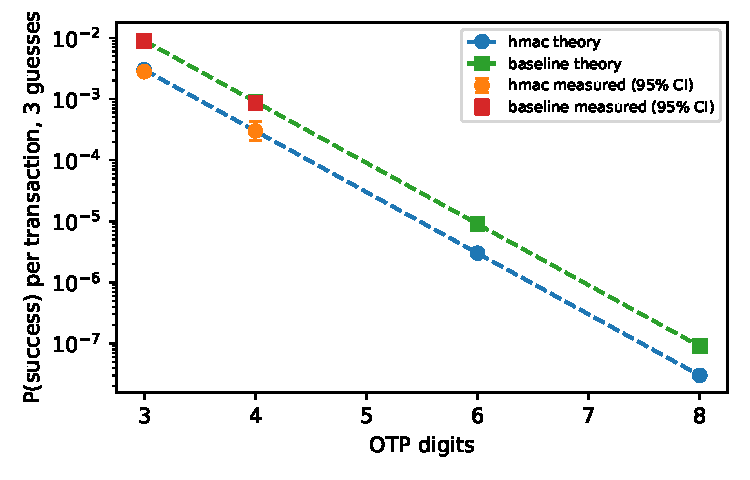
\includegraphics[width=0.75\linewidth]{figures/bruteforce.pdf}
\caption{Empirical vs theoretical guessing probability (F5).}
\label{fig:bruteforce}
\end{figure}

\paragraph{Limitation of G4 (per-transaction only).}
The three-attempt limit is per transaction; there is no per-user counter and
transaction creation is not rate-limited (\cref{sec:threat}). An attacker with
the password but no phone can create $k$ transactions and guess three times each.
Modelling the attempts as independent, the cumulative success probability is
\[
  P_k = 1-(1-p)^k \approx k\cdot p \quad\text{when } k\,p \ll 1,
\]
where $p$ is the per-transaction probability of \cref{tab:bruteforce}. Solving
$P_k=\tfrac12$ gives $k=\ln 2/\!\ln(1/(1-p))\approx (\ln 2)/p$: roughly
$7.7\times10^{4}$ transactions for a 50\% chance against \texttt{baseline}
(6 digits, $p\approx9.0\times10^{-6}$) and about $2.3\times10^{7}$ against
\texttt{hmac} (8 digits, $p=3.0\times10^{-8}$). This is an idealised bound that
assumes the valid-code window stays fixed over the campaign; for \texttt{baseline}
the TOTP code rotates every $30$~s, so tens of thousands of transactions inside a
single window is not a realistic, measured capability --- only the
per-transaction probabilities in \cref{tab:bruteforce} are measured. For
\texttt{sig}/\texttt{sig\_blind} guessing does not apply: random forgery of an
ECDSA signature is computationally infeasible. The \cmark{} for G4 therefore means only that
the per-transaction lockout works. A per-user or per-device failure counter and a
rate limit on transaction creation would close the gap, at the cost of letting an
attacker who knows the password lock the victim out on purpose (a denial of
service).

\subsection{Server compromise and verifiable evidence}
\label{sec:eval-dbleak}
Scenarios S10 and S11 separate \texttt{hmac} from \texttt{sig}. In S10 the
attacker holds a copy of the database and tries to forge a transfer. Because the
server stores $K_{\text{totp}}$ and $K_{\text{hmac}}$ in the clear (deliberately,
to make this scenario real), an attacker with the database can compute valid
\texttt{baseline} and \texttt{hmac} codes --- so both are \xmark{}. The signing
key, by contrast, is generated on the phone and never exported, so the database
does not contain the ECDSA private key (it still holds sessions and the symmetric
keys) and \texttt{sig}/\texttt{sig\_blind} remain \cmark{}. S10 evaluates leakage
of device key data while the enrolled device remains unchanged. A real system
would protect the symmetric keys in an HSM; we did not, in order to demonstrate
exactly this difference.

S11 asks whether a third party can verify the stored evidence. For
\texttt{baseline} and \texttt{hmac} the evidence is a symmetric OTP, checkable
only by whoever holds the key, so the answer is \emph{no}. For \texttt{sig} the
evidence is a signature any party can verify with the public key, so the answer
is \emph{yes}. For \texttt{sig\_blind} the answer is \emph{yes} with the
asterisk: the signature proves the device signed, not that the user saw the
transaction. As set out in \cref{sec:threat}, this is \emph{verifiable evidence},
not non-repudiation: the authenticator is served by the bank, and the public key
is attested by no independent party.

\subsection{Summary against security goals}
\Cref{tab:goalsummary} collapses the scenario matrix onto the seven goals
(generated by \texttt{make scenarios}).

\begin{table}[htbp]
\centering
\caption{Security goals met by each mode (T6). Source: derived from
\texttt{results/scenarios.csv}.}
\label{tab:goalsummary}
\small
% --- begin generated content (results/goals.tex) ---
\begin{tabularx}{\linewidth}{@{}lXcccc@{}}
\toprule
Goal & Description & baseline & hmac & sig & sig\_blind \\
\midrule
G1 & Authorization integrity (code bound to the exact transaction) & \xmark & \cmark & \cmark & \cmark \\
G2 & Freshness (no replay, no late use) & \cmark & \cmark & \cmark & \cmark \\
G3 & Single use under concurrency & \cmark & \cmark & \cmark & \cmark \\
G4 & Guessing limit per transaction & \cmark & \cmark & \cmark & \cmark \\
G5 & Resilience to server database leak & \xmark & \xmark & \cmark & \cmark \\
G6 & Verifiable evidence (third party can check) & \xmark & \xmark & \cmark & \cmark$^{*}$ \\
G7 & What you see is what you sign (attentive user) & \xmark & \cmark & \cmark & \xmark \\
\bottomrule
\end{tabularx}
\par\smallskip{\footnotesize $^{*}$ In \texttt{sig\_blind} the signature only proves that the device signed, not that the user saw the transaction.\par}
% --- end generated content ---
\end{table}
